\documentclass[10 pt]{article}

\usepackage{fontspec}
\defaultfontfeatures{Mapping=tex-text}
\setmainfont{Minion Pro}

%\usepackage{graphicx}
%\usepackage{fullpage}

\usepackage{lastpage, fancyhdr}
\pagestyle{fancy}
\lhead{Scott O'Connor}
\chead{Ancient Philosophy} 
\rhead{\emph{Meno}}
\lfoot{}
\cfoot{\thepage\space of \pageref{LastPage}} 
\rfoot{}



\begin{document}
\author{Ancient Philosophy}
\title{\emph{Meno}}

\section*{Overview}
The dialog begins with (M)eno, a Thessalian, asking (S)crates whether virtue is teachable (70a1-4). M is politically ambitious, young, handsome, well-born, and visiting Athens with Anytus, one of S's prosecutors, as a host.  M will embark on a controversial military and political career that ends with his young death by the Persian king.  

`Virtue' translates `arete', but it's an imperfect translation. The difficulty is best introduced by analogy. There is a difference between the excellent and mediocre boxer, the excellent and mediocre ice-skater, the excellent and mediocre university student, etc. The Greeks believed that just as you could excel in some specific activity, you could excel at being human. You could be an excellent human or a merely mediocre human. `Arete' is here used to describe whatever is needed to excel at something. There is, then, an arete of a boxer, which is  different from the arete of an ice-skater.  There is also the arete of excellent human beings, which is what allows us excell being human. `Virtue' was the standard translation of `arete', but that was complicated when `virtue' becomes restricted to a set of moral qualities that included chastity, temperance, etc.

Greeks wanted to become and be excellent humans. They dedicated their time and resources to attain virtue, and they placed a very high value on its teachability.  Famous poets, speakers, politicians, generals, etc., claimed they could teach it; students and their families paid hefty sums for that. So to ask whether virtue is teachable, as M asks S, is a very controversial question. Answering `no' is risky.  

Unsurprisingly, S claims he doesn't know the answer to M's question because he, S, does not know what virtue is (71b1--8). `What X is' is a complicated phrase. S is interested in the \emph{ti esti} of virtue. This phrase is translated as `essence' and `nature' in English. The English word  is itself derived from the Latin `essentia', which was an artificial word formed by the Latin `esse' introduced especially to comment on our Greek phrase. So, S claims we must first answer the question `what is the essence of virtue?' before we can determine whether virtue is teachable. An answer to such a question is called a Socratic Definition. S, therefore, is here assuming the following principle: 
\begin{description}
\item[The priority of definition:] In order to know what qualities X possesses, you must know the essence of X, i.e., you must know the Socratic definition of X. 
\end{description}
Since S does not know the essence of virtue, he does not know its qualities, including whether it is teachable. The dialog proceeds by discussing  various candidate definitions of virtue. During this initial discussion, S again illustrates the requirements for a Socratic definition. He does so in two ways. First, he asks M to define virtue and illustrates the requirements by failure. Second, he gives a few successful definitions of color. This tells M how he should define virtue. We again learn that an adequate definition must be a) general, b) univocal, and c) explanatory. 

%An objection: S claims that to know whether M is good-looking, rich, or well-born, you must know who M is.  If you do not know at all who M is, then you cannot know what qualities belong to M. This seems implausible. Suppose I see a red-haired stranger. Can I not know that the person has red hair without knowing who they are? S might respond by asking what we mean by saying that we know that the person has red hair. Assume that the person's name is John. If I do now know who John is, then S will claim that I cannot know that John has red hair. I can know, perhaps, that there is a person in a room with red hair. But that is quite different from knowing that \emph{John has red hair}. Since I don't know that the person is John, I couldn't know that John has red hair. 

 The dialog takes a tangent, which is our focus. M argues that inquiry into the nature of things is impossible. S's response will teach us about S's epistemology, about how he believes that he can inquire into, and help others inquire into, the nature of those things that he does not yet know. 

\section*{The paradox of inquiry}
Let us assume that the priority of definition is true. If you do not know the essence of  X, it follow that you do not know any of X's qualities. Thus, if you do not know the essence of X, you are in a complete blank regarding X. M grows frustrated with S's demands for a definition and argues that we cannot inquire into the essence of X if we are in a complete blank regarding X (80d5-80e5). 

\begin{enumerate}
\item[P1.] If you know [essence of] X already, you cannot inquire into [essence of] X. 
\begin{itemize}
\item When people begin searching for something, they do not yet possess what they are searching for. So if they did already possess something, it makes no sense to search for it.
\end{itemize}
\item[P2.] If you do not know [essence of] X, you cannot inquire into [essence of] X.\begin{enumerate}
\item If you do not know \emph{at all} what X is, then you cannot start to inquire into the essence of X...you will not know how to start even looking.
\item If you do not know \emph{at all} what X is, and if you stumble upon X, you will not know that what you stumbled upon is X, e.g., if you do not know who M is, but stumble upon him, then you will not know that the person you stumbled upon is M. 
\end{enumerate}
\item[P3.] Either you know [essence of]  X or you do not know [essence of] X...(implicit premise) 
\item[C.] You cannot inquire into [essence of] X.
\end{enumerate}
Impasse!  S claimed that we cannot find out whether virtue is teachable until we know the essence of virtue.  But M argues that we cannot inquire into the essence of virtue if we know nothing at all about it. This is a serious impasses. It seems we must know at least something about virtue before we can investigate its essence. But it also seems that we cannot know anything about virtue without already knowing its essence.  

\section*{The Theory of Recollection (TR)}
To solve the dilemma, S must feasibly reject at least one of the premises. We will see that he rejects P2. His core claim is that ``what we call learning is recollecting things we already know (81b3--c9).'' This is called \emph{The Theory of Recollection (TR)} because it claims that learning is merely recollecting what one used to know but subsequently forgot. 

In order to defend TR, S engages with one of M's slaves. S's goal is to show that 1) the child can learn something he doesn't know by recollecting it, i.e., he learns/recollects the lengths of each side of a 8 sq ft square (85d2-10). 2) S does not possess the knowledge that the child acquires, and, thus, can help the child inquire even though he does not have the relevant knowledge they both seek. 


%Before we look at the details, consider how this might solve the paradox. S seems to distinguish between latently knowing and explicitly knowing something. He subsequently endorses these two claims:  

%\begin{enumerate}
%\item We cannot inquire into what we \emph{explicitly} know, but \emph{we can} inquire into what we \emph{latently} know. 
%\item We cannot inquire into what we do not even \emph{latently} know, but \emph{we can} inquire into what we do not \emph{explicitly} know.
%\end{enumerate}


S asks the child various questions about geometry. The child claims to have knowledge, S cross-examines him, and the child then confesses \emph{puzzlement}; thereafter the child gets it right by applying his own reasoning, not by bowing to S's authority. This supposedly proves TR for the following reasons: 

\begin{itemize}
\item If the child can give correct answers, he must, in some sense, know the answers. 
\item The child has not learned geometry before. 
\item The child was not taught any geometry by S in their exchange--so the child didn't \emph{learn} it then either.
\begin{itemize}
\item Since S does not himself have the answers, he cannot be teaching them to the child. 
\item S claims that his questions merely elicit the child's \emph{beliefs}. 
\end{itemize}
\item We need some explanation of why the child, through his discussion with S, will reliably \emph{reject} false beliefs and \emph{accept} true beliefs. 
\item S claims that this is possible because the child (like everyone) once knew (in a disembodied state) but forgot, and hence can recognize the truth, and so reject the false.
\item S claims that the child \emph{will} know it through further questioning.
\end{itemize}
 
\noindent \emph{Question about TR:} What kinds of truths does S think we can recollect?
\begin{enumerate}
\item He clearly allows geometrical truths (and so mathematical truths generally?). 
\item He should allow ethical truths (including truths about value) (otherwise the unity of the dialogue would be in jeopardy). 
\item He also suggests nature ``as a whole''?---What could that mean?\item What about empirical truths? 
\end{enumerate}
 
 

\section*{True belief vs. knowledge}
S allows that inquiry into X is possible by possessing true opinions about X. Thus, you can inquire into what you do not know as long as you have true opinions about the target of your inquiry. TR shows us that recollections provide us with true opinions. It is left open whether recollection is the only way to acquire such opinions. This solution introduces a distinction between \emph{doxa} and \emph{episteme}. The former is translated as both `belief' and `opinion'. The latter is translated as `knowledge' and sometimes `understanding'. 

What's the difference? After the exchange, M insists that S address whether virtue is teachable, despite S's demand to determine what virtue is first. S again refuses to address that question directly, but instead notes that if virtue is knowledge, then virtue will be teachable (and if virtue is not knowledge, it will not be teachable). He then turns his attention to the question whether virtue is knowledge, considering arguments for and against.
\begin{itemize}\item{The main \emph{pro} argument is that, since virtue is beneficial, and all actions guided by knowledge turn out well, virtue must be knowledge}
\item S maintains that they were right to say that actions guided by knowledge always turn out correctly, BUT
\item They were wrong to say that \emph{only} actions guided by knowledge turn out correctly---actions guided by true opinion (\emph{doxa}) also turn out correctly

\begin{itemize}\item{The example of the ``Road to Larissa'' (97a5-c2) is supposed to show this}\end{itemize}

\item This leads M to ask ``why knowledge (\emph{epist\^{e}m\^{e}}) is prized far more highly than right opinion, and why they are different'' (97d1-2)

\item S answers that right opinion is ``upgraded'' into knowledge by a ``giving an account of the reason why'' (i.e. by working out the explanation of the relevant fact) which ``ties'' the opinion to the soul. Knowledge is more valuable because it remains in place.
\item Those with knowledge succeed all the time. Those with true opinion succeed only some of the time.

\end{itemize}

\noindent \emph{Differences between belief and knowledge:} 

\begin{enumerate}
\item If S believes P, it does not follow that P is true. There can be true and false beliefs. 
\item If S knows P, P is true. There cannot be false knowledge.
\item If S believes P, it does not follow that S possesses the explanation for P (alternatively, it does not follow that S is justified in believing P). There are both rational and irrational beliefs.
\item If S knows P, then (i) S believes P, (ii) P is true, and (iii) S possess the explanation for P (alternatively, S is justified in believing P). 
\item If S believes P and P is true, it does not follow that S knows P.  
\end{enumerate}

For example, just because the child has true beliefs about geometry, it does not follow that the child has knowledge about geometry. Just because a person has true beliefs about biology, it does not follow that the person has knowledge about biology. Just because a person believes truly that God exists (or God does not), it does not follow that that person know that God exists (or God does not). Finally, just because Socrates has true beliefs about virtue, it does not follow that Socrates has knowledge about virtue. 

 



\end{document}

What do you think, Meno? Has he, in his answers, expressed any opin- ion that was not his own?
No, they were all his own.
And yet, as we said a short time ago, he did not know?- That is true.
So these opinions were in him, were they not? -Y es.
So the man who does not know has within himself true opinions about
the things that he does not know'?-So it appears.
These opinions have now just been stirred up like a dream, but if he
were repeatedly asked these same questions in various ways, you know that in the end his knowledge about these things would be as accurate as anyone's.-It is likely.

If then, during the time he exists and is not a human being he will have
true opinions which, when stirred by questioning, become knowledge, will not his soul have learned during all time? For it is clear that during all time he exists, either as a man or not. - S o it seems.86

%\section*{The discussion}

%\begin{enumerate}
%\item The slave is said to have no geometrical knowledge before the discussion (85e)
%\item S claims that he has not taught the slave anything during their discussion
%\begin{itemize}\item{S is probably working with a conception of ``teaching'' on which for S to teach X that P would be for X to come to believe that P \emph{only because} S tells X that P}\end{itemize}
%\item But, by the end of the discussion, the slave has the opinion that the double-area square comes to be from the diagonal of the original square
%\begin{itemize}\item{So, given [2], S asks where that opinion came from}\item{S claims that it must have been, in some sense, in the slave already (85c)}\end{itemize}
%\item S claims that the slave, at the end of the discussion, does not yet have \emph{epist\^{e}m\^{e}} of the geometrical fact, but that the slave \emph{will} acquire it through further questioning (85c7-d4)
%\item Since that further questioning will not violate [2], S concludes that the slave will acquire the knowledge ``from himself by himself''
%\item The phenomenon described in [5] is claimed to be an instance of ``recollection'' (\emph{anamn\^{e}sis})
%\item So, S takes himself to have answered the paradox of inquiry by showing that the slave can go from a state of not having \emph{epist\^{e}m\^{e}} (at least, not explicitly) to a state of having \emph{epist\^{e}m\^{e}} (i.e. explicitly). And, he maintains that it is because the slave once knew, then forgot, and through questioning can be made to recollect, that successful inquiry is possible. 
%\end{enumerate}






\section*{True belief vs. knowledge}

After the exchange, M insists that S address whether virtue is teachable, despite S's demand to determine what virtue is first. S again refuses to address that question directly, but instead notes that if virtue is knowledge, then virtue will be teachable (and if virtue is not knowledge, it will not be teachable). He then turns his attention to the question whether virtue is knowledge, considering arguments for and against.
\begin{itemize}\item{The main \emph{pro} argument is that, since virtue is beneficial, and all actions guided by knowledge turn out well, virtue must be knowledge}
\item S maintains that they were right to say that actions guided by knowledge always turn out correctly, BUT
\item They were wrong to say that \emph{only} actions guided by knowledge turn out correctly---actions guided by true opinion (\emph{doxa}) also turn out correctly

\begin{itemize}\item{The example of the ``Road to Larissa'' (97a5-c2) is supposed to show this}\end{itemize}

\item This leads M to ask ``why knowledge (\emph{epist\^{e}m\^{e}}) is prized far more highly than right opinion, and why they are different'' (97d1-2)

\item S answers that right opinion is ``upgraded'' into knowledge by a ``giving an account of the reason why'' (i.e. by working out the explanation of the relevant fact) which ``ties'' the opinion to the soul. Knowledge is more valuable because it remains in place.

\item Question: What has \emph{not} been done in the discussion with the slave such that further questioning could lead the slave to work out the explanation of the geometrical theorem?

\item Question: S seems to allow that inquiry into X is possible by possessing true opinions about X. How does this fit with his response to the paradox of inquiry, which, we recall concerned knowledge? Is he claiming that you can inquire into what you do not know as long as you have true opinions about the target of your inquiry? Might that mean that the theory of recollection is not needed to solve the paradox? Or is Socrates telling us merely that recollections provides us with true opinions?
\end{itemize}


%\section*{How natures can play an explanatory role}

%\noindent Euclid's \emph{Elements} Book 1, Proposition 34: In parallelogrammic figures the opposite sides and angles are equal to one another, and \emph{a diagonal cuts them in half}

%\noindent And, [F1] since the point A is the center of the circle CDB, [F2] AC is equal to AB.

%\begin{figure}[h!]
%\centering
%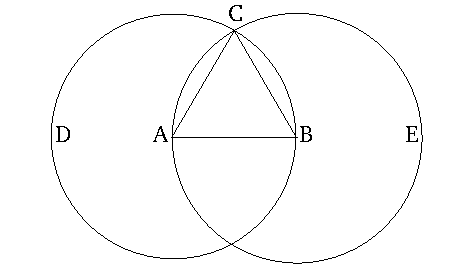
\includegraphics[scale=0.7]{circle}
%\caption{}
%\label{fig:prop 34}
%\end{figure}

%\noindent Definition of Circle: A Circle is a plane figure contained by one line, such that all of the straight-lines falling upon it from one point among those lying within the figure are equal to one another



